\documentclass{beamer}
%\usecolortheme{seahorse} % change this
\usepackage{graphicx}
\usepackage{inconsolata}
\usepackage{anyfontsize}
\usepackage{courier}
\usepackage{color}


\usepackage{natbib} 
%bibstyle muss einer da sein, 
% setimmt wie der kram an \cite aussieht.
% https://de.wikibooks.org/wiki/LaTeX-W%C3%B6rterbuch:_bibliographystyle
%https://de.sharelatex.com/learn/Bibtex_bibliography_styles
%\bibliographystyle{abbrvnat} 
%\bibliographystyle{unsrt} 
\bibliographystyle{plainnat}

%gets rid of bottom navigation bars
\setbeamertemplate{footline}[frame number]{}

%gets rid of bottom navigation symbols
\setbeamertemplate{navigation symbols}{}

%gets rid of footer
%will override 'frame number' instruction above
%comment out to revert to previous/default definitions
\setbeamertemplate{footline}{}

\newcommand{\red}[1]{\textcolor{red}{#1}}
\definecolor{darkgreen}{RGB}{42, 158, 50}
\newcommand{\green}[1]{\textcolor{darkgreen}{#1}}

\title 
{Generative adversarial training on \\ structured domains}
\author % NEEDS MOAR INFO ,, contact etc
%{Stefan Mautner }
{\underline{Stefan Mautner} \and Fabrizio Costa 
    \small{ 
        \texttt{
            \href{mailto:mautner@informatik.uni-freiburg.de}
            {mautner@informatik.uni-freiburg.de}
        }
        \texttt{
            \href{mailto:f.costa@exeter.ac.uk}
            {f.costa@exeter.ac.uk}
        }
   }
}

\date 
%{Freiburg University \\2017-04-10}

\titlegraphic{
\includegraphics[width=2cm]{images/logo.jpg}
}

\begin{document}
\frame{\titlepage}



% design goals
\begin{frame}
\frametitle{Constructive Machine Learning}

    \begin{itemize}
        \item {\bf What:} answer \red{design} questions using examples
        \item We are interested in: \\
        constructive approaches for \red{structured} domains
        \item In chemo- and bio-informatics: \\
        synthesize molecules with a desired bio-activity
    \end{itemize}
    \begin{figure}
        \centering
        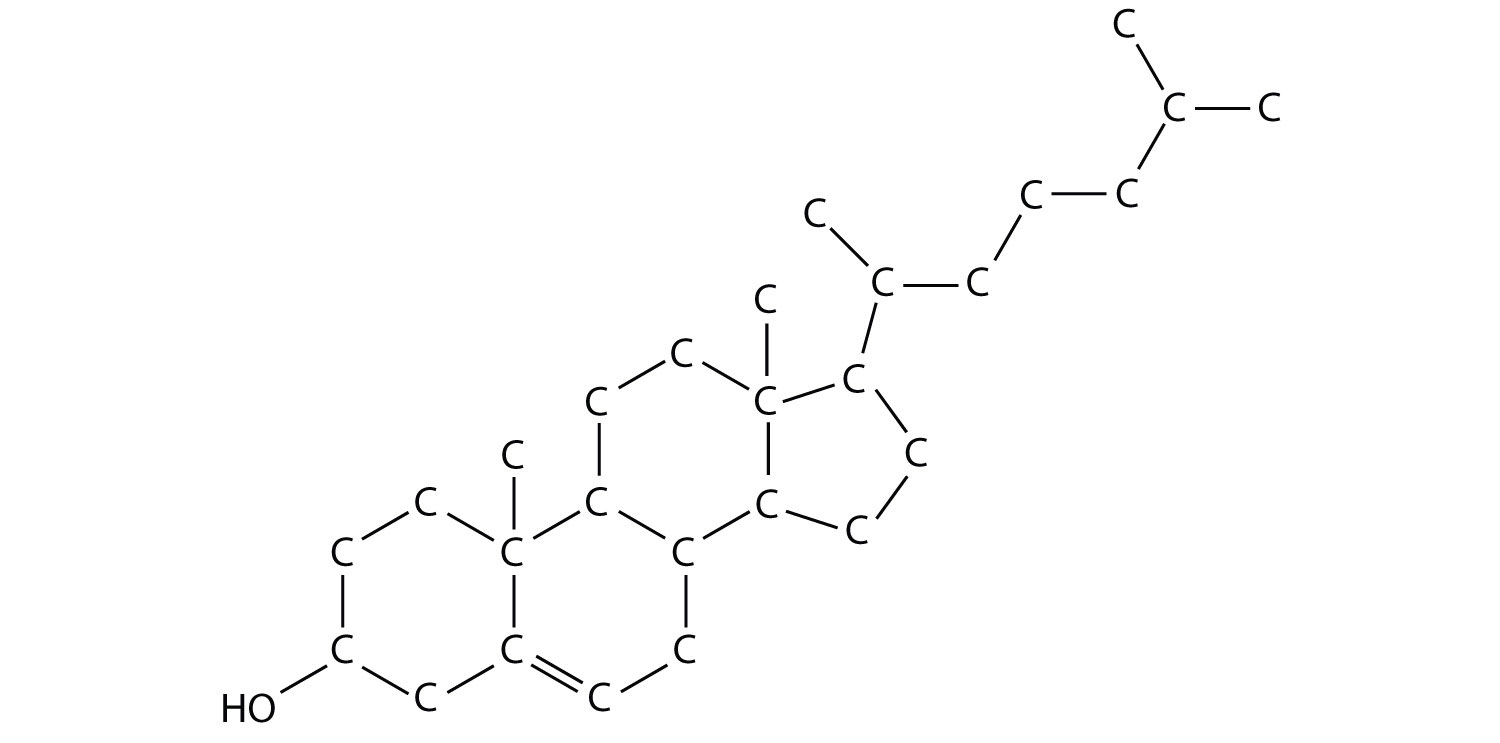
\includegraphics[width=0.5\textwidth]{images/mol.jpg}
        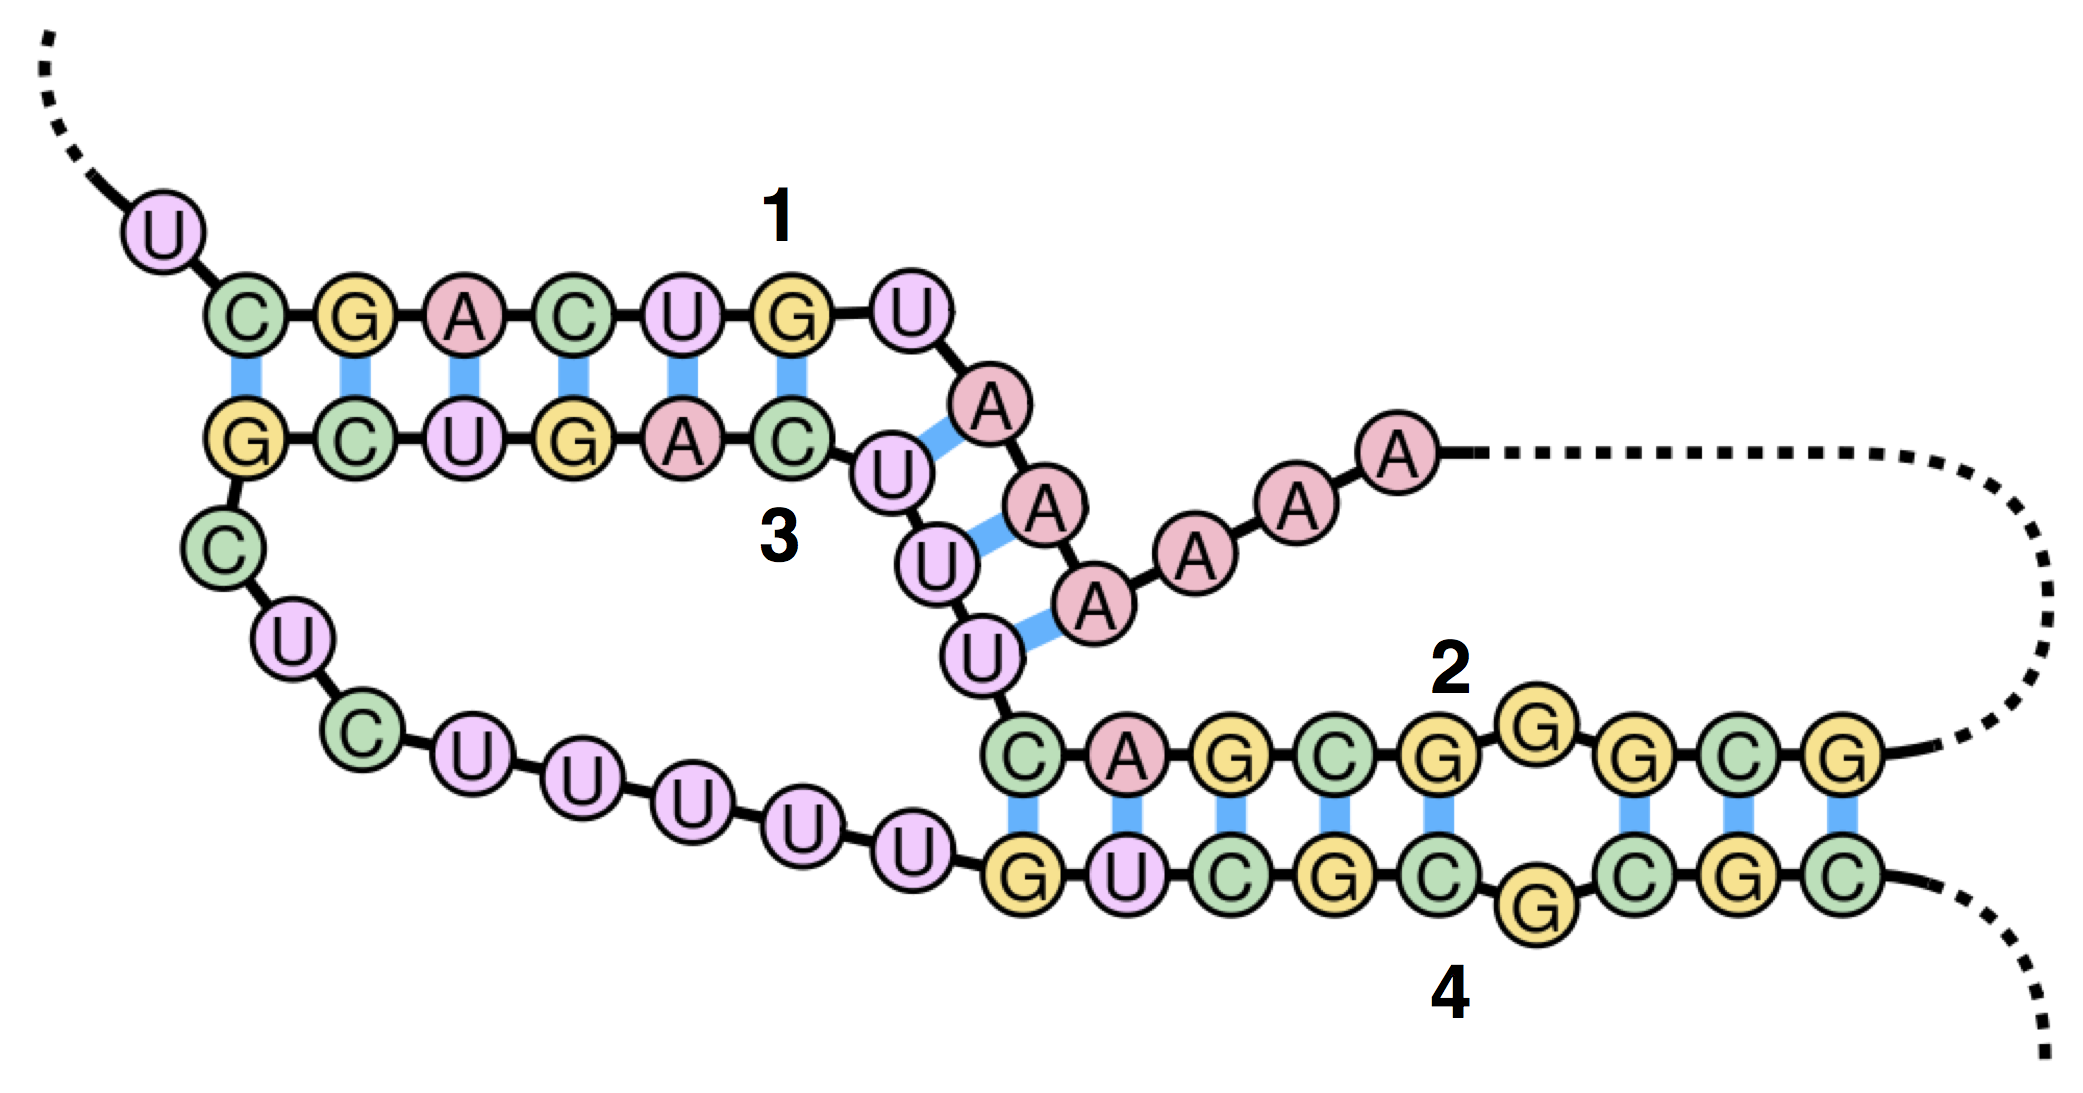
\includegraphics[width=0.5\textwidth]{images/rna.png}
    \end{figure}    
\end{frame}




%%%%%%%%%%%%%%%%%%%%%%%%%%%%%%%%%%%%%%%%%%%%%%%%%%%%%%%%%%%%%%%%%%%%%%%%%%%%
% add iverview slide... 

\begin{frame}
\frametitle{Assumed work}
    \begin{itemize}
        \item EDeN (Explicit Decomposition with Neighborhoods)\footnote{github.com/fabriziocosta/EDeN}
        \begin{itemize}
            \item Vectorizes Graphs
            \item Used when training models from graphs
            \item (not discussed here)
        \end{itemize}    
    
    \item GraphLearn \footnote{github.com/fabriziocosta/GraphLearn} 
        \begin{itemize}
            \item generates instances given examples
            \item (overview given here)
        \end{itemize}    
        \item This is a sampling extension for GraphLearn
    \end{itemize}    

\end{frame}
%%%%%%%%%%%%%%%%%%%%%%%%%%%%%%%%%%%%%%%%
\begin{frame}
\frametitle{The Problem}
    \begin{itemize}
        \item Density estimation based on observed graphs (preferably few, "positive"
            class only)
        \item Implies loose constraints on feasible manyfold\\
            $\rightarrow$ negative impact on generated instances
        \item \red{Question}: How tighten constraints?
            %a: Generative adversarial training
    \end{itemize}
    \begin{figure}[ht]
        \centering
        \footnote{ Yann Le Cun, NIPS 2016 Keynote (modified)}
        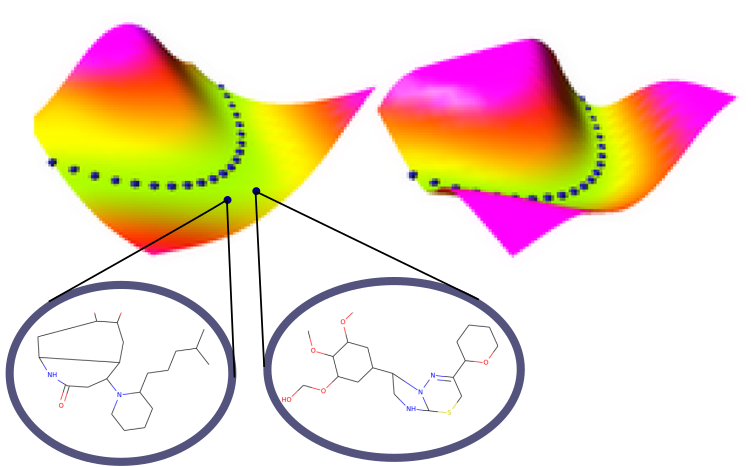
\includegraphics[width=0.8\textwidth]{images/valley.png}
    \end{figure}    
\end{frame}



\begin{frame}
\frametitle{Generative ANN architectures}
    \begin{itemize}

        \item Fully visible belief networks (FVBNs)
        \item Variational autoencoders
        \item \red{Generative adversarial networks GANs}

            %\red{ === gans developed in this comunity .. generative pictures}
    \end{itemize}

    %\begin{itemize}
    %    \item say something about gans
    %\end{itemize}

    \begin{figure}[ht]
        \centering
        \footnote{Al Gharakhanian,  Blogpost, Dec 2016}
        \includegraphics[width=0.6\textwidth]{images/GAN.png}
        \footnote{Ian Goodfellow, NIPS 2016}
        \includegraphics[width=0.2\textwidth]{images/fabann.png}
    \end{figure}   
\end{frame}



%\begin{frame}
%\frametitle{GAN examples}
%    \begin{figure}[ht]
%        \centering
%        \footnote{Legid \emph{et al.} 2016}
%        \includegraphics[width=0.7\textwidth]{images/GAN2.png}
%    \end{figure}   
%    \begin{figure}[ht]
%        \centering
%        \footnote{github.com/mattya/chainer-DCGAN }
%        \includegraphics[width=0.7\textwidth]{images/animee.png}
%    \end{figure}   
%\end{frame}



\begin{frame}
\frametitle{GAT on structured domains}
    \begin{itemize}
            % why the new thing should work etc then proposal.
            % comes from NN etc now we use GAN for structures

            % shpere with data drawing... regions where dots are dense and undense
            % but 1class says things are ok if above plane..
            % arrow to undense region -> point to bad graphs
        %\item To generate instances, \red{we} require a model 
        %\item There might not be enough train data to capture the densities correctly. 
        \item The graph generation guiding model might be not tight enough
        \item ANN researchers inspired us by addressing  a very similar problem using GANs
        %\item use gen instances to train better discriminators
        %\item use made graphs and make increatingly good graphs 4 graphs
        
        \item {\bf Proposal:} Generate instances and assume they are negative examples
            to \red{improve} the generation guiding model
    \end{itemize}
    \begin{figure}[ht]
        \centering
        \includegraphics[width=0.7\textwidth]{images/valley_x3_stars.png}
    \end{figure}    
\end{frame}

%%%%%%%%%%%%%%%%%%%%%%%%%%%%%%%%%%%%%%%%%%%%%%%%%%%%%%%%%%%%%%%%%%%%%%%%%%%%

\begin{frame}
\frametitle{The constructive learning problem for finite samples\footnote{Costa Artif. Intell. 2016}}
    \begin{itemize}
        \item Given a set of graphs $G$
        \item use a parametrized generator $M_\theta$ to \red{construct} set $G_\theta$
        \item find optimal $\theta$ to \red{jointly} satisfy:
            \begin{enumerate}
        \item probability density is the \red{same} if estimated over $G$ or $G_\theta$
        \item $G_\theta$ \red{differs} from $G$
            \end{enumerate}
        \item Optimize:\\ \begin{center} $\arg \min_\theta L(P(G),P(G_\theta)) + \lambda  ~ Sim(G, G_\theta)$ \end{center}
        \item where:
        \begin{itemize}
            \item $L$ is a loss over probability distributions \\(e.g. symmetric Kullback Leibler divergence)
            \item $Sim$ is a {\em set} graph kernel
            \item $\lambda$ is desired trade off
        \end{itemize}
    
    \end{itemize}
    %$${argmin}_{\theta}~~L(f_{G_0}(G),f_{G_{\theta}}(G))+\lambda \frac{K(G_0,G_{\theta})}{\sqrt{K(G_0,G_0),K(G_{\theta},G_{\theta})}}}$$
\end{frame}




% so far we have the basic graphlearn
\begin{frame}
    \frametitle{Parametrized Generator for Graphs}
    \begin{itemize}
        \item Instead of generating $\mapsto$ \red{sample} from a corresponding probability distribution over graphs
        \item We use Metropolis Hastings (MH) \begin{tiny}Markov Chain Monte Carlo (MCMC)\end{tiny}
        \begin{enumerate}
            \item start from {\em seed} graph $x$
            \item propose according to $g(x \mapsto x')$
            \item accept according to: \\
            \begin{center}
            $A(x \mapsto x')=\min(1, \frac{P(x')}{P(x)} \frac{g(x \mapsto x')}{g(x' \mapsto x)})$
            \end{center}
        \end{enumerate}
        \item {\bf Q:} how not to reject proposed graphs too often?
        \item {\bf A:} use graph \red{grammar} induced from data  for $g(x \mapsto x')$
    \end{itemize}
\end{frame}

\begin{frame}
    \frametitle{Graph Grammar}
    A graph grammar is a finite set of productions P=(M,D,E) 
    \begin{itemize}
        \item M=mother graph
        \item D=daughter graph
        \item E=embedding mechanism
    \end{itemize}
    \begin{figure}[ht]
        \centering
        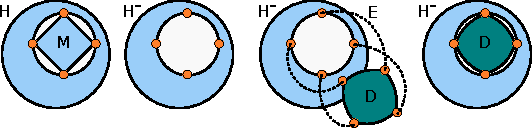
\includegraphics[width=0.9\textwidth]{images/grammar.pdf}
    \end{figure}
\end{frame}

%\begin{frame}
%    \frametitle{Substitutable Graph Grammar}
%    \begin{itemize}
%        \item \red{cores} (neighborhood graphs) can be substituted..
%        \item .. if they have the same \red{interface} graph
%    \end{itemize}
%    \begin{figure}[ht]
%        \centering
%        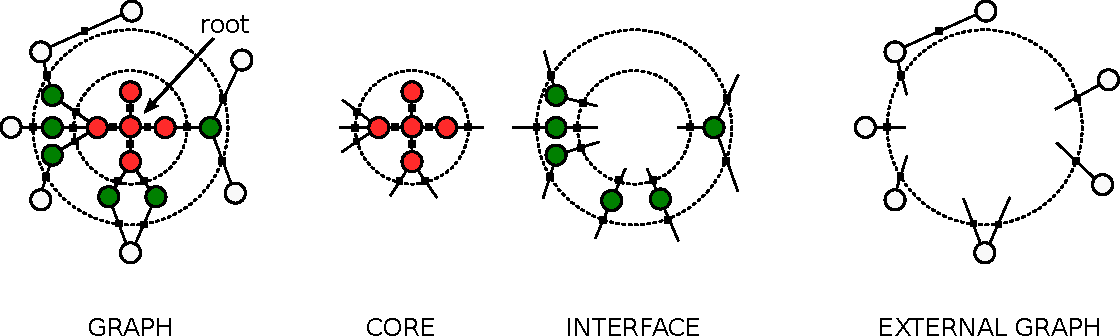
\includegraphics[width=0.9\textwidth]{images/cip1.pdf}
%    \end{figure}
%\end{frame}

\begin{frame}
    \frametitle{Substitutable Graph Grammar}
    \begin{itemize}
        \item \red{cores} (neighborhood graphs) can be substituted 
..
        \item .. if they have the same \green{interface} graph
    \end{itemize}
    \begin{figure}[ht]
        \centering
        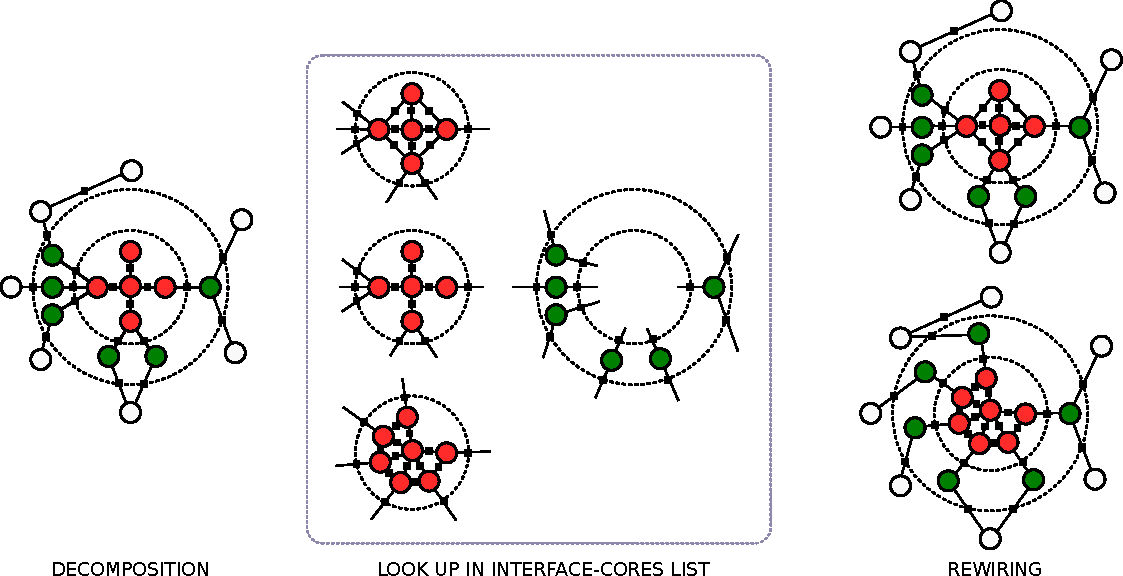
\includegraphics[width=0.9\textwidth]{images/cip2.pdf}
    \end{figure}
\end{frame}



% write about ze new algo :)

\begin{frame}
    \frametitle{Generative adversarial training}

\begin{figure}[ht]
       \centering
      \includegraphics[width=0.3\textwidth]{images/valley_x3_stars.png}
\end{figure}   
  
    Input: \emph{train}; a set of observed  instances
    \begin{enumerate}
            % IMPROVE THIS name of sets need change
            % also show that previous gens are used

        \item train \red{one class} model on \emph{train}
        \item use \emph{train} as seeds for generation
        \item train \red{two class} model on \emph{train} (classlabel 1) \\
            and all generated instances (classlabel 0)
        \item use \emph{train} as seeds for generation
        \item goto 3
    \end{enumerate}
    \begin{figure}[ht]
        \centering
        \includegraphics[width=0.5\textwidth]{images/genmod_recol.png}
    \end{figure}
\end{frame}


% show that each generation the graphs get betta?

% BENCHMARK II
\begin{frame}
    \frametitle{Training accuracy on internal models}
    \begin{itemize}
        \item Are generated instances similar to the observed instances?
    \end{itemize}

   \begin{figure}[ht]
        \centering
        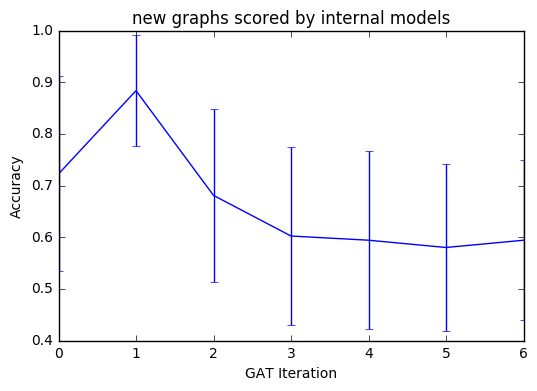
\includegraphics[width=0.70\textwidth]{images/eval2.png}
        \footnote{500 graphs in train set, 3 repeats, pubchem aid 651610}
    \end{figure}
   \small{\em lower accuracy indicates that the sets are becoming harder to separate}
\end{frame}

% BENCHMARK I 
\begin{frame}
    \frametitle{Test accuracy on internal model}
    \begin{itemize}
            % new headlines for all pictures
            % fir linear regressor  or quadratic
            % make first and last datapoints visible 
        \item Is the observed class actually learned?
            \footnote{note that the training process has never seen any real
            negative instances}
    \end{itemize}

   \begin{figure}[ht]
        \centering
        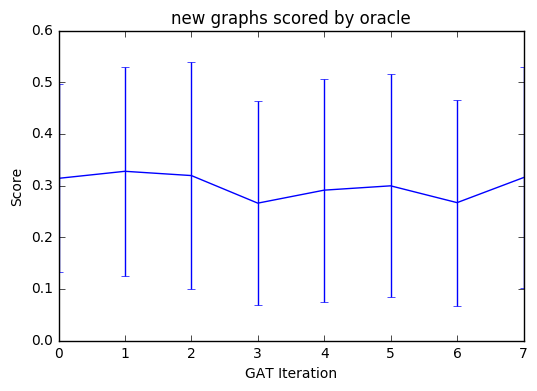
\includegraphics[width=0.70\textwidth]{images/eval3.png}
    \end{figure}
    \small{\em  Lower training accuracy coincides with higher test accuracy}
   %\small{\em scores above horizontal dotted line indicate reliable identification}
\end{frame}



\begin{frame}
    \frametitle{Conclusion}
    \begin{itemize}
        \item  Generative adversarial training effective in tightening 
            generation contrains
        \item Test on larger data set required
    \end{itemize}

    %\begin{itemize}
    %\end{itemize}
\end{frame}



% OWARI DA 
%\begin{frame}
%    \frametitle{Thank You}
%    
%    %\begin{itemize}
%    %    \item  Thank you
%        %\item {\bf Future work:} \\\red{learn} task specific coarsening strategy directly from data   
%    %\end{itemize}
%    \begin{figure}[ht]
%        \centering
%        \includegraphics[width=0.6\textwidth]{images/grp.png}
%    \end{figure}
%    
%    \begin{itemize}
%        \item  Greetings from Freiburg :D
%        %\item {\bf Future work:} \\\red{learn} task specific coarsening strategy directly from data   
%    \end{itemize}
%    %\begin{itemize}
%    %\end{itemize}
%\end{frame}


% BENCHMARK III
%\begin{frame}
%    \frametitle{Evaluation III}
%    \begin{itemize}
%        \item Objective quality of designs \red{THIS IS STILL BAD}
%    \end{itemize}
%
%   \begin{figure}[ht]
%        \centering
%        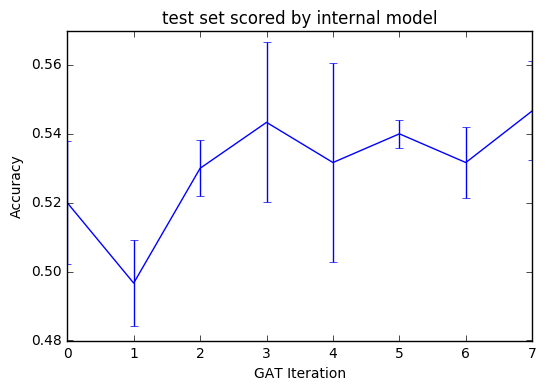
\includegraphics[width=0.80\textwidth]{images/eval1.png}
%    \end{figure}
%   %\small{\em scores above horizontal dotted line indicate reliable identification}
%\end{frame}



\end{document}
